%!TEX root = ../article.tex

\section{BlendMe! - The User Study}
\label{sec:blendme}

\subsection{Objectives}
%
The goals which we have picked for this User Study were to \ul{understand if color blendings
can be detected by users}, \ul{is it easier for users to estimate the pair of colors
that resulted in a particular given blend, or reciprocally, to estimate which blend will
result from a given pair of colors}, \ul{to detect if the users follow some kind of mental
convention and organize the color when conveying the answers}, and formulate possible
implications of color blending usage, in Information Visualization field of research. \par
%
We have planned to develop this study in two different strands: in a \textbf{Laboratory
Environment}, which will allow us to calibrate and perfectly control the entire study
conditions, and in an \textbf{Online Environment}, which will allow us to disseminate our
study to a larger set of users. Therefore, we have defined the following questions:
%
\begin{itemize}
	\item \textbf{Q1:} Which Color Model best meets the users' expectations, when
  blending two colors?
	\item \textbf{Q2:} Do users specify the Blending-basis following some order, when
  users are indicating possible color mixtures' results?
	\item \textbf{Q3:} Are there evidences from differences across demographic groups, such
  as the age or gender?
\end{itemize}
%
We drafted our study into four different phases: a \textbf{User Profiling Phase},
a \textbf{Calibration Phase}, a \textbf{Color Deficiency Test Phase} and finally, the
\textbf{Core Phase}. In the following section, we detail each of these study phases.
%
\subsection{Design}
%
We intended to develop a user study which could support the laboratory controlled
environment, while at the same time supporting the collection of metrics and data from the
online users: this is an important consideration, since the workload when analyzing the
results would be dramatically reduced because the data is condensed and gathered in the same
fashion, and data would be more comparable. When brainstorming the ideas for this study, we started
with the intention of testing both the blending of two colors and three colors; we decided that the
colors which would be blended were Red (\textbf{R}), Green (\textbf{G}), Blue (\textbf{B}), Cyan
(\textbf{C}), Magenta (\textbf{M}) and Yellow (\textbf{Y}), since they represent each primitive of
the most commonly known Color Models, \ul{RGB (Additive Color Model)} and \ul{CMYK (Subtractive Color Model)}.
The color models we intended to study: the color models were \textbf{HSV, RGB, CMYK, CIE-L*a*b*} and
\textbf{CIE-L*C*h*}. \par
%
Then, we produced a wide spreadsheet of possible blendings of these colors, according to these color models,
\textbf{mixed in pairs of two colors}: this generated the total amount of 78 blendings, \textbf{There are
15 possible mixtures of two colors}, when combining the previous defined colors: R-G, R-B, G-B, R-C, R-M,
R-Y, C-M, M-Y, G-C, G-M, G-Y, B-C, B-M, B-Y and C-Y. Since we wanted to \textbf{test if it is better to give
the result already mixed, or indicate the blending-basis and the users create the color mixture}, we developed
a set of 32 questions to present to the user: 17 of them are of the type \textbf{presenting the resulting
color, and ask for the blending-basis}, and 15 of them are of type \textbf{given the blending-basis, ask for
the blending-result}. The entire set of questions is mapped in Table \ref{table:color_blendings}.
%
\begin{table}[htbp]
	\centering
  \resizebox{0.45\textwidth}{!} {
	\begin{tabular}{cc|ccc}
		\hline
		                              & Given the Result, Asked for Basis                       &                               & \multicolumn{2}{c}{Given the Basis, Asked for Result}                                                                                                       \\ \cline{2-2} \cline{4-5}
		\multirow{-2}{*}{Question ID} & Given Color                                             & \multirow{-2}{*}{Question ID} & \multicolumn{2}{c}{Given Colors}                                                                                                                            \\ \hline
		\multicolumn{1}{c|}{1}        & \cellcolor[HTML]{FFFF00}\#FFFF00                        & \multicolumn{1}{c|}{18}       & \multicolumn{1}{c|}{\cellcolor[HTML]{FF0000}{\color[HTML]{FFFFFF} \#FF0000}} & \multicolumn{1}{c|}{\cellcolor[HTML]{00FF00}\#00FF00}                        \\ \hline
		\multicolumn{1}{c|}{2}        & \cellcolor[HTML]{FF00FF}\#FF00FF                        & \multicolumn{1}{c|}{19}       & \multicolumn{1}{c|}{\cellcolor[HTML]{FF0000}{\color[HTML]{FFFFFF} \#FF0000}} & \multicolumn{1}{c|}{\cellcolor[HTML]{0000FF}{\color[HTML]{FFFFFF} \#0000FF}} \\ \hline
		\multicolumn{1}{c|}{3}        & \cellcolor[HTML]{80FF00}\#80FF00                        & \multicolumn{1}{c|}{20}       & \multicolumn{1}{c|}{\cellcolor[HTML]{00FF00}\#00FF00}                        & \multicolumn{1}{c|}{\cellcolor[HTML]{0000FF}{\color[HTML]{FFFFFF} \#0000FF}} \\ \hline
		\multicolumn{1}{c|}{4}        & \cellcolor[HTML]{7F00FF}{\color[HTML]{FFFFFF} \#7F00FF} & \multicolumn{1}{c|}{21}       & \multicolumn{1}{c|}{\cellcolor[HTML]{FF0000}{\color[HTML]{FFFFFF} \#FF0000}} & \multicolumn{1}{c|}{\cellcolor[HTML]{00FFFF}\#00FFFF}                        \\ \hline
		\multicolumn{1}{c|}{5}        & \cellcolor[HTML]{FF0080}{\color[HTML]{FFFFFF} \#FF0080} & \multicolumn{1}{c|}{22}       & \multicolumn{1}{c|}{\cellcolor[HTML]{FF0000}{\color[HTML]{FFFFFF} \#FF0000}} & \multicolumn{1}{c|}{\cellcolor[HTML]{FF00FF}\#FF00FF}                        \\ \hline
		\multicolumn{1}{c|}{6}        & \cellcolor[HTML]{FF8000}\#FF8000                        & \multicolumn{1}{c|}{23}       & \multicolumn{1}{c|}{\cellcolor[HTML]{FF0000}{\color[HTML]{FFFFFF} \#FF0000}} & \multicolumn{1}{c|}{\cellcolor[HTML]{FFFF00}\#FFFF00}                        \\ \hline
		\multicolumn{1}{c|}{7}        & \cellcolor[HTML]{0000FF}{\color[HTML]{FFFFFF} \#0000FF} & \multicolumn{1}{c|}{24}       & \multicolumn{1}{c|}{\cellcolor[HTML]{00FFFF}\#00FFFF}                        & \multicolumn{1}{c|}{\cellcolor[HTML]{FF00FF}\#FF00FF}                        \\ \hline
		\multicolumn{1}{c|}{8}        & \cellcolor[HTML]{FF0000}{\color[HTML]{FFFFFF} \#FF0000} & \multicolumn{1}{c|}{25}       & \multicolumn{1}{c|}{\cellcolor[HTML]{FF00FF}\#FF00FF}                        & \multicolumn{1}{c|}{\cellcolor[HTML]{FFFF00}\#FFFF00}                        \\ \hline
		\multicolumn{1}{c|}{9}        & \cellcolor[HTML]{00FF80}\#00FF80                        & \multicolumn{1}{c|}{26}       & \multicolumn{1}{c|}{\cellcolor[HTML]{00FF00}\#00FF00}                        & \multicolumn{1}{c|}{\cellcolor[HTML]{00FFFF}\#00FFFF}                        \\ \hline
		\multicolumn{1}{c|}{10}       & \cellcolor[HTML]{0080FF}{\color[HTML]{FFFFFF} \#0080FF} & \multicolumn{1}{c|}{27}       & \multicolumn{1}{c|}{\cellcolor[HTML]{00FF00}\#00FF00}                        & \multicolumn{1}{c|}{\cellcolor[HTML]{FF00FF}\#FF00FF}                        \\ \hline
		\multicolumn{1}{c|}{11}       & \cellcolor[HTML]{FF8000}\#FF8000                        & \multicolumn{1}{c|}{28}       & \multicolumn{1}{c|}{\cellcolor[HTML]{00FF00}\#00FF00}                        & \multicolumn{1}{c|}{\cellcolor[HTML]{FFFF00}\#FFFF00}                        \\ \hline
		\multicolumn{1}{c|}{12}       & \cellcolor[HTML]{80FF00}\#80FF00                        & \multicolumn{1}{c|}{29}       & \multicolumn{1}{c|}{\cellcolor[HTML]{0000FF}{\color[HTML]{FFFFFF} \#0000FF}} & \multicolumn{1}{c|}{\cellcolor[HTML]{00FFFF}\#00FFFF}                        \\ \hline
		\multicolumn{1}{c|}{13}       & \cellcolor[HTML]{0080FF}{\color[HTML]{FFFFFF} \#0080FF} & \multicolumn{1}{c|}{30}       & \multicolumn{1}{c|}{\cellcolor[HTML]{0000FF}{\color[HTML]{FFFFFF} \#0000FF}} & \multicolumn{1}{c|}{\cellcolor[HTML]{FF00FF}\#FF00FF}                        \\ \hline
		\multicolumn{1}{c|}{14}       & \cellcolor[HTML]{8000FF}{\color[HTML]{FFFFFF} \#8000FF} & \multicolumn{1}{c|}{31}       & \multicolumn{1}{c|}{\cellcolor[HTML]{0000FF}{\color[HTML]{FFFFFF} \#0000FF}} & \multicolumn{1}{c|}{\cellcolor[HTML]{FFFF00}\#FFFF00}                        \\ \hline
		\multicolumn{1}{c|}{15}       & \cellcolor[HTML]{00FF80}\#00FF80                        & \multicolumn{1}{c|}{32}       & \multicolumn{1}{c|}{\cellcolor[HTML]{00FFFF}\#00FFFF}                        & \multicolumn{1}{c|}{\cellcolor[HTML]{FFFF00}\#FFFF00}                        \\ \hline
		\multicolumn{1}{c|}{16}       & \cellcolor[HTML]{FF007F}\#FF007F                        & \multicolumn{3}{c}{}                                                                                                                                                                        \\ \cline{1-2}
		\multicolumn{1}{c|}{17}       & \cellcolor[HTML]{00FF00}\#00FF00                        & \multicolumn{3}{c}{\multirow{-2}{*}{}}                                                                                                                                                      \\ \cline{1-2}
	\end{tabular}}
  \vspace{+5pt}
  \caption{Two types of questions asked about Color Blendings}
  \label{table:color_blendings}
\end{table} \par
%
\subsubsection{User Profiling}
%
In these phase, questions were asked about the Age, Gender, Academic Degree, Nationality and Country of Residence:
these questions helped us conceiving user profiles with key indicators about cultural background and gender
relation to results of each test.%
%
\subsubsection{Testing Calibration}
%
We developed another solution for remote controlling the calibration on the \ul{online environment}: to present
two similar calibration images, one presenting a set of shaded squares ranging from grey to black shades against
a black background, and another presenting instead white squares against a white background. The iser had to
indicate the number and word from the last square which he could easily see. This information provide us input
about the white-level and black-level of the screen, which are nothing more than the \textbf{Contrast} and \
textbf{Brightness}, respectively, of the display. Regarding the \ul{laboratory environment}, we conducted the
users tests in a LCD monitor which was calibrated using a Spyder\footnote{"Spyder - Datacolor Imaging Solutions",
Available at: \url{http://spyder.datacolor.com}. Last accessed on October 17th, 2016.} Colorimeter, that will
consider the existing light in the environment and adjust the color of each pixel to a standard. \par
%
\subsubsection{Testing Color Vision Deficiencies}
%
The Color Deficiency Test was comprised of a set of six plates, which were able to detect which type of color
vision deficiencies the user would eventually have. This test in commonly known as the \emph{Ishihara Test},
which has a validated \cite{Alwis1992} short form that rearranges the order in which the plates are presented.
We have only chosen plates which detect color vision deficiencies in the Red-Green field, since it is the most
common deficiency. The plates chosen were:
%
\begin{itemize}
	\item \ul{Plate \#1} - Presents the number \textbf{12}. Every user should be capable of viewing the same number.
	\item \ul{Plate \#2} - Presents the number \textbf{29} for regular users which do not have any color vision
  deficiency, and the number \textbf{70} to users which have \ul{a deficiency in the Red-Green field}.
	\item \ul{Plate \#3} - This plate is a confirmation from the result of the previous one, presenting \textbf{74}
  to regular users and \textbf{21} to users which have \ul{a deficiency in the Red-Green field}.
	\item \ul{Plate \#4} - Presents the number \textbf{45} for the regular users, and the ones which have a
  color vision deficiencies are supposed to see a blob.
	\item \ul{Plate \#5} - Presents the number \textbf{26} for the regular users, the ones which have
  \ul{Deuteranopia see only the number \textbf{2}} and the ones which have \ul{Protanopia see number \textbf{6}}.
	\item \ul{Plate \#6} - Presents the number \textbf{35} for the regular users, the ones which have
  \ul{Deuteranopia see only the number \textbf{3}} and the ones which have \ul{Protanopia see number \textbf{5}}.
\end{itemize}
%
\subsubsection{Core Test}
%
This phase is the principal part of the study, which will evaluate the \textbf{Blending of Two Colors}. We have
composed an interface with a small set of objects which would be used and interacted with to provide the colors
to the user, and receive his input values, among other objects. We wanted to provide a tool which would be
capable of displaying without being influenced by its surrounding of even by the proximity of other colors: then
the colors were presented in rounded shapes, accompanied by what we call \emph{\textbf{color sliders}} whenever
it was needed input colors from the user. With this, only the necessary colors are displayed on the circles as
the users wish and there is no interference of undesired colors, allowing us to eliminate the influence of them. \par
%
These shapes start filled with an empty color (or white) so it \textbf{does not influence color perception},
and the users are not influenced by previously used colors, when answering to another question. There is no
particular reason for the chosen shapes are circles, since \textbf{we are not studying the best visualizations
to convey information, when using color blending techniques}. \par
%
The most interesting fact of this test phase is how the color slider works: we chose the HSV Color Model to
represent the colors to show, since the \textbf{HSV Color Model has the best compromise when presenting colors
in information visualization} because of its primitives (Hue, Saturation and Value). \textbf{We have chosen to
only modify the Hue value and leave the Saturation and Value on its maximum value}: this way, we could ensure
that we could present the entire range of colors at its full saturation and value, also simplifying the gathering
of values from the users. Therefore, the color slider yields a value within the range of $[0º ; 360º]$ degrees
which corresponds to an angle in the Hue circle of the HSV Color Model. Moreover, the scale of values of the
slider, though representing continuous angle values, does not presents the values ordered from 0º to 360º.
Instead, \textbf{fixed intervals of values are mixed within each other}, so the users do not formulate any
mental organization in the moment and do not demonstrate any previous conception or mindset. A representation
of these color sliders in present in Figure \ref{fig:sliders}, which depicts a wireframe version of these
objects.
%
\begin{figure}[htbp]
	\centering
  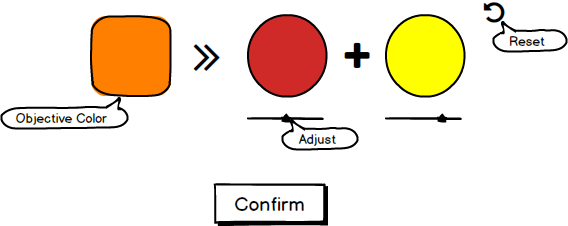
\includegraphics[width=0.45\textwidth]{images/sliders.png}
  \caption{Wireframe of Color Sliders}
  \label{fig:sliders}
\end{figure} \par
%
The colors represented in the shapes and the ones present in the pre-calculated answers have a particularity,
in the laboratory environment: these pre-calculated values are, with the help of a \emph{Matlab} script,
going to be \textbf{converted to adapted color values, according to the .icc color profile file generated by
the Spyder Colorimeter}. This way, we guarantee that no matter if the laboratory environmental conditions
change, the colors will always be presented equally to every user. \textbf{This script processes each possible
result for every color pair, in every color model}, converts it to a normalized CIE-XYZ value and in the end,
to an hexadecimal color code to be printed on the shapes of the interface, when time comes for the laboratory
user to choose a color from the color slider. This process was realized before each user session. \par
%
After the users indicated and confirms their answer, \textbf{they were presented a satisfaction question with
a 5-point Likert Scale} to double-check the easiness of each mixture, as Gama and Gonçalves did \cite{Gama20141}.
